\section{Gestion des mati{\`e}res}

Voici les diff{\'e}rents sc{\'e}narios:\\

\section*{Enseignant}

\begin{center}
\scalebox{0.6}{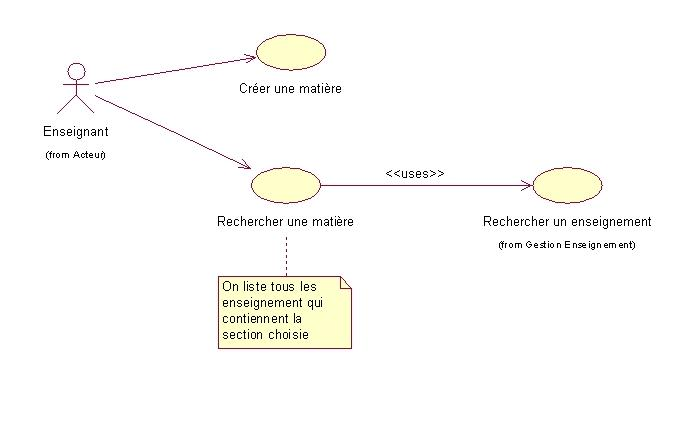
\includegraphics{images/Matiere_Enseigant.jpg}}\\
\end{center}

\begin{tabular}{|p{4cm}|c|p{4cm}|p{5cm}|}
\hline
  Fonction & Priorit{\'e} & Qualit{\'e} & Mesure \\
\hline
cr{\'e}er une mati{\`e}re & 4 & Fiable, Facile & Pas de redondance. Ergonomique.\\
\hline
Rechercher une mati{\`e}re & 4 & Rapide et Complet & Permet de lister l'ensemble des enseignements qui contiennent la mati�re.\\
\hline
\end{tabular}

\begin{center}
{\'e}chelle de mesure de la priorit{\'e}:

\scalebox{0.5}{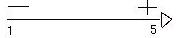
\includegraphics{images/echelle.jpg}}
\end{center}

\begin{itemize}
\item  {\bf Cr{\'e}er une mati{\`e}re :}
	\begin{itemize}
	\item Pr{\'e}-requis : Etre log{\'e} 
	\item Description :Il s'identifie avec son login et son mot de passe. \\
	Il saisie la nouvelle mati{\`e}re et valide.
	\item Post-requis : Une nouvelle mati{\`e}re est cr{\'e}{\'e}e si elle n'existait pas.\\
	\end{itemize}

\item  {\bf Rechercher une mati{\`e}re :}
	\begin{itemize}
	\item Pr{\'e}-requis : Etre log{\'e} et cr{\'e}ateur de la section.
	\item Description : Il s'identifie avec son login et son mot de passe.\\
	L'utilisateur demande le contenu d'une mati�re.\\
	On liste tous les enseignements qui contiennent cette mati�re.
	\end{itemize}

\end{itemize}

\section*{Administrateur}

\begin{center}
\scalebox{0.6}{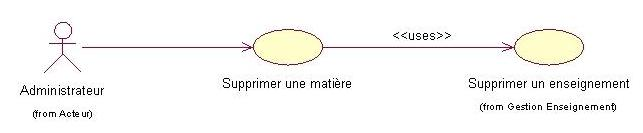
\includegraphics{images/Matiere_Administrateur.jpg}}\\
\end{center}

\begin{tabular}{|p{4cm}|c|p{4cm}|p{5cm}|}
\hline
  Fonction & Priorit{\'e} & Qualit{\'e} & Mesure \\
\hline
Supprimer une mati�re & 4 & Fiable, Facile & On ne doit pas pouvoir effacer une mati�re qui a encore des liens avec un enseignement.\\
\hline
\end{tabular}

\begin{center}
{\'e}chelle de mesure de la priorit{\'e}:

\scalebox{0.5}{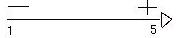
\includegraphics{images/echelle.jpg}}
\end{center}

\begin{itemize}
\item  {\bf Supprimer une mati�re :}
	\begin{itemize}
	\item Pr{\'e}-requis : Etre log{\'e} 
	\item Description :Il s'identifie avec son login et son mot de passe. \\
	Il s�lectionne une mati�re contenue dans aucun enseignement.\\
	Il clique l'option {\it Suppression} et valide son choix.
	\item Post-requis : La mati�re est supprim�e.
	\end{itemize}
\end{itemize}
